
\begin{definition}
Una \emph{función entre dos conjuntos numéricos}, A conjunto inicial y B conjunto final, es una correspondencia por la cual a cada elemento de un subconjunto de A, llamado \emph{dominio de la función} y denotado por $Dom(f)$, le corresponde un elemento y sólo uno de un subconjunto de B, llamado \emph{imagen} o \emph{recorrido de f}, y denotado por $Im(f)$.\\
Una función se puede representar por:
$$
\begin{array}{rcl}
	f:A &\longrightarrow & B \\
	x & \mapsto & f(x)
\end{array}
$$
\end{definition}

Ejemplo de representación gráfica de una función:
\geogebra{bm9zpgfh}

\subsubsection{Clasificación de funciones}
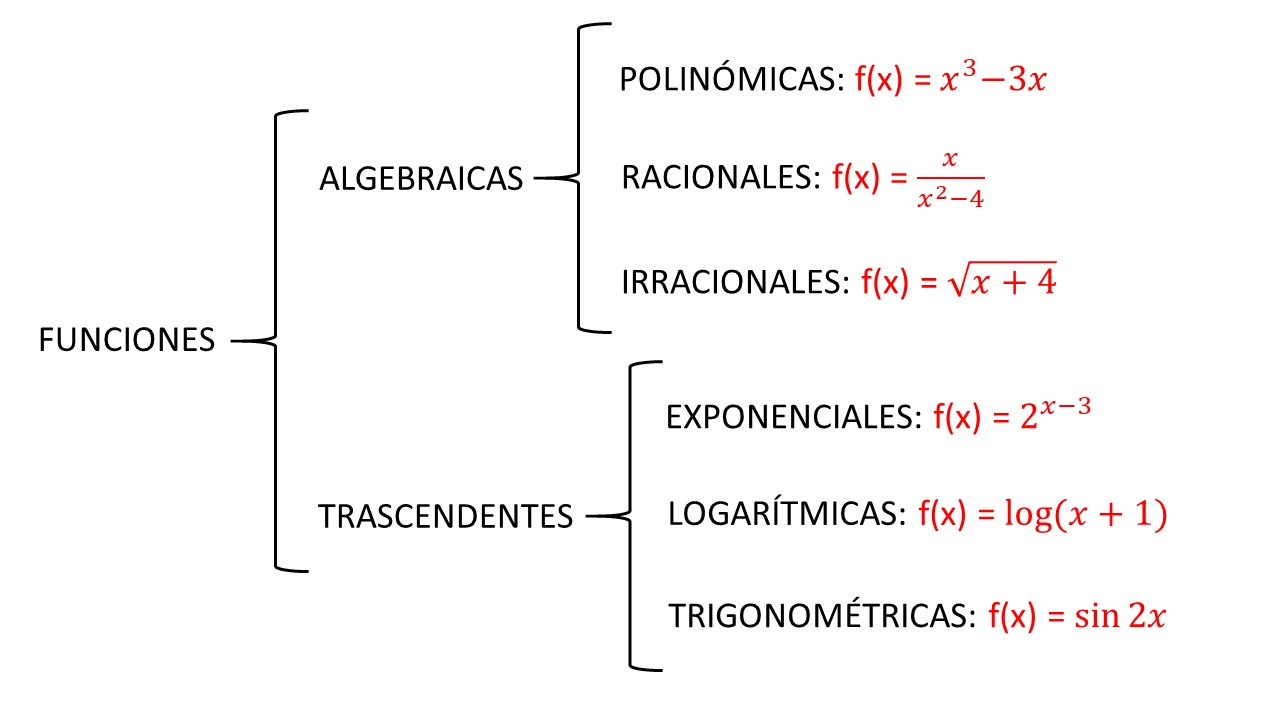
\includegraphics[width=40cm, height=20cm]{samples/propiedades/clasificaEsquema2.jpg}
\subsubsection{Ejemplos}
\begin{itemize}
	\item \textbf{Polinómicas.}
	$f(x) = x^3-3x$
	\geogebra{cwt7r5f7}
	\item \textbf{Racionales.}
	$f(x) = \dfrac{x}{x^2-4}$
	\geogebra{cdwjf88d}
	\item \textbf{Irracionales.}
	$f(x) = \sqrt{x+4}$
	\geogebra{xjn6vrn8}
	\item \textbf{Exponenciales.}
	$f(x) = 2^{x-3}$
	\geogebra{faj4urcm}
	\item \textbf{Logarítmicas.}
	$f(x) = \ln (x-1)$
	\geogebra{apzz89ae}
	\item \textbf{Trigonométricas.}
	$f(x) = \sin(2x)$
	\geogebra{yvw8jubg}
\end{itemize}

\subsubsection{Dominio}
\begin{definition}
	El \emph{dominio de una función real}, también llamado \textbf{dominio de definición} o \textbf{campo de existencia}, es el conjunto de los elementos para los cuales la función está definida. Dicho de otra manera, es el subconjunto de números reales que tienen imagen.
	$$Dom_{f} =\{x \in R / \exists y = f(x) \in \mathbb{R}\}$$
\end{definition}
\begin{itemize} 
	\item $\mathbf{Dom_{f}}$: dominio de la función. También se puede denotar por $Dom(f)$ o, simplemente, $D$. Puede ser todo el conjunto de los números reales, o buen un subconjunto de este: $Dom_{f} \subseteq R$. 
	\item $\mathbf{x}$: número real, perteneciente al dominio de la función, que recibe el nombre de variable independiente. 
	\item $\mathbf{y}$: número real, perteneciente al conjunto e la imagen de la función, recibe el nombre de variables dependiente. Para obtener su valor se debe aplicar la función $f$ al valor de $x: f(x)=y$. Para un par de valores concretos $(x,y)$ se dice que $y$ es la \textbf{imagen} de $x$, y que $x$ es la \textbf{antiimagen} de $y$.
\end{itemize} 
\youtube{lmfDEGDpgV8}
\subsubsection{Cómo calcular el dominio}
Para calcular el dominio "eliminaremos" de la ecuación aquellos valores que hagan imposible realizar alguna operación matemática.
\begin{itemize}
	\item \textbf{Funciones polinómicas}\\
	El dominio de toda función polinómica es $\mathbb{R}$, ya que al sustituir un número real cualquiera $x \in R$, siempre va a existir $f(x)$.
	\item \textbf{Funciones racionales}\\
	El \textbf{denominador} debe de ser \textbf{diferente de cero}. Suponiendo una función $f(x) = \dfrac{P(x)}{Q(x)}$, si tanto $P(x)$ como $Q(x)$ son polinomios, entonces el dominio $Dom_{f}= \{x \in R / Q(x) \neq 0\}$, es decir, el conjunto de valores que \textbf{no anulan} el denominador.\\
	Cuando simplifiques una función racional, el dominio debe coincidir con el de la función original, y no debes caer en la tentación de recalcularlo.
	\item \textbf{Funciones irracionales}\\
	\begin{itemize}
		\item \emph{Función irracional de índice impar}\\
		En estos casos, la raíz no impone ninguna restricción adicional al dominio, por lo que coincidirá con el del radicando.
		\item \emph{Función irracional de índice par}\\
		En estos casos la raíz impone que los valores del radicando siempre sean mayores o iguales que cero.
	\end{itemize}
	\item \textbf{Funciones exponenciales}\\
	En estos casos, la exponencial no impone ninguna restricción adicional al dominio, con lo que coincidirá con el dominio del exponente.
	\item \textbf{Funciones logarítmicas}\\
	En estos casos el logaritmo impone que el argumento debe de ser un número positivo.
	\item \textbf{Funciones trigonométricas}\\
	El dominio de las funciones del tipo $f(x)=\sin[g(x)]$ y $f(x)=\cos[g(x)]$, es el dominio de $g(x)$. Las funciones del tipo $f(x)=\tan[g(x)]$ tienen por dominio:
	$$Dom(f)=\{x \in \mathbb{R} | g(x) \neq \dfrac{\pi}{2} + k\pi \text{, } k \in \mathbb{Z}\}$$	
\end{itemize}

\subsubsection{Ejercicios.}
\begin{ex}[sol after]
	Rellene las siguientes definiciones:
		\begin{itemize}
			\item Una \emph{función} es una ............. tal que a cada valor del ........ conjunto le corresponde un ......... valor del ........... conjunto.	
		\end{itemize}
	\begin{sol}
		\begin{itemize}
			\item Una función es una \emph{correspondencia} tal que a cada valor del \emph{primer} conjunto le corresponde un \emph{único} valor del \emph{segundo} conjunto. 
		\end{itemize}
	\end{sol}
\end{ex}

\vspace{1cm}


\begin{ex}[sol later]
	Introduzca en la barra de entrada las siguientes funciones, de manera similar a la indicada en el ejemplo anterior, y observa la gráfica de representación de cada una de las funciones.
	\begin{itemize}
		\item $f(x) = 3x+2$
		\item $g(x) = \dfrac{x^2-3}{x+5}$
		\item $h(x) = \sqrt{x+5}$
		\item $j(x) = \dfrac{2x^2+1}{3x-5}$
		\item $k(x) = \log (x^2)$
		\item $p(x) = 3\cos(3x)$
	\end{itemize}
	\begin{sol}
		\geogebra[ai=true, stb=true]{tc5pbmae}
	\end{sol}
\end{ex}

\vspace{1cm}

\begin{ex}[sol later]
	Calcula el dominio de las siguientes funciones a partir de la teoría explicada previamente:\\
	\begin{itemize}
		\item $f(x) = \dfrac{2x}{3x-2}$
		\item $f(x) = \dfrac{6x}{x^2-16}$
		\item $f(x) = \sqrt{x^2-1}$
		\item $f(x) = \sqrt{\dfrac{3}{-x+2}}$
		\item $f(x) = \sqrt{\dfrac{x+5}{x-7}}$
		\item $f(x) = \sqrt{x^2+x}$
		\item $f(x) = \log(-2x^2-10x-8)$
		\item $f(x) = \arccos(x+5)$
		\item $f(x) = e^x$
		\item $f(x) = e^{-5x}$
	\end{itemize}
	\begin{sol}
		\begin{itemize}
			\item $\mathbb{R}-\{\dfrac{2}{3}\}$
			\item $\mathbb{R}-\{-4, 4\}$
			\item $(-\infty, -1]\bigcup [1, +\infty])$
			\item $(-\infty, 2)$
			\item $(-\infty, -5]\bigcup [7, +\infty])$
			\item $(-\infty, -1]\bigcup [0, +\infty])$
			\item $(-4,-1)$
			\item $[-6, -4]$
			\item $\mathbb{R}$
			\item $\mathbb{R}$
		\end{itemize}
	\end{sol}
\end{ex}

\vspace{1cm}

\begin{ex}[sol after]
	Comprueba mediante la representación en la gráfica que los dominios que has calculado coinciden con lo que se observa en las gráficas.
	\begin{sol}
		\geogebra[ai=true, stb=true]{tc5pbmae}
	\end{sol}
\end{ex}
